\documentclass[a4paper,11pt,oneside]{article}
\usepackage[T1]{fontenc}
\usepackage[latin1]{inputenc}
%\usepackage{ae}
%\usepackage{ngerman}
%\usepackage{epsfig}
%\usepackage{float,graphicx,graphics}
\usepackage[dvips]{graphicx}
\usepackage{wrapfig}
\usepackage{capt-of}

\usepackage{lscape}
\usepackage{fancyvrb}
\usepackage{fancyhdr}
\usepackage{multicol}
\usepackage{amssymb} 
\usepackage{amsmath} 

\usepackage[bf]{caption2}
\renewcommand{\captionfont}{\small\itshape}

\usepackage[
        a4paper,      % A4
        dvips,        % Erzeugung durch dvips
        pdftitle={LDAPCon 2009 - The Apache Directory Project: Toolchain for Developers},
        bookmarks=true,
        bookmarksnumbered=true, % Verwendete Bookmarks anzeigen
%        colorlinks,   % Farbige Links
        linkcolor=blue,
        urlcolor=blue,
        citecolor=blue]{hyperref}
\usepackage[dvips]{thumbpdf}

\usepackage{vmargin}
\setpapersize{A4}

\setmargins{2.5cm}{2.5cm}% % linker & oberer Rand
           {16cm}{25cm}%   % Textbreite und -hoehe
           {0pt}{0pt}%   % Kopfzeilenhoehe und -abstand
           {0pt}{0pt}%    % \footheight (egal) und Fusszeilenabstand

\usepackage{setspace}
\onehalfspacing  % anderthalbzeilig
%\doublespace     % doppelzeilig 

\setlength{\parindent}{0cm}
%\setlength{\parskip}{0.2cm}
\setlength{\parskip}{1ex plus 0.5ex minus 0.2ex}
\setlength{\fboxsep}{0.2cm}
\pagestyle{fancy}
\lhead{}
%\headheight = 25.3pt

% \setlength{\parindent}{0pt}

\pagestyle{empty}

\begin{document}

\thispagestyle{empty}
\begin{Huge}
\noindent
\textbf{The Apache Directory Project - } \\
\textbf{Toolchain for Developers} \\
\end{Huge}

by Stefan Seelmann \\

%\newpage
%\tableofcontents
%\newpage
\section{Introduction}
LDAP is widely adopted; directory servers like Active Directory or OpenLDAP are often used as central user repository. However many developers are not familiar with LDAP because of fear or dislike of its complexity. One very likely reason is the lack of tooling. One aim of the Apache Directory project is to provide solutions and tools to make LDAP more convenient for developers. This paper will introduce the tools provided by the Apache Directory project and will show how these can help application developers to integrate LDAP into their applications.


\section{Tool Overview}

The Apache Directory project consists of two major sub-projects: Server and Studio.

\subsection{Apache Directory Studio}
Apache Directory Studio is a LDAP client platform. It is based on Eclipse and extends it with several plugins:
\begin{itemize}
\item The LDAP Browser Plugin is a tool for browsing, searching and editing entries present in an LDAP Server.
\item The LDIF Editor Plugin can be used to edit LDIF files. It provides syntax highlighting and context assistance.
\item The Schema Editor Plugin is intended to design and edit the Schema of an LDAP Server (object classes and attribute types).
\item The Configuration Plugin for Apache DS can be used to edit the configuration file of the Apache Directory Server.
\item The ApacheDS Plugin provides an integrated LDAP server within Apache Directory Studio.
\end{itemize}

These plugins can be installed into an existing Eclipse using the update site. Developers who are familiar with Eclipse will experience a seamless integration into their IDE. There are also installers and tar balls for Mac OS, Linux and Windows available to run Apache Directory Studio as a standalone application.

Apache Directory Studio leverages the Eclipse platform (Views, Editors, Wizards, Jobs-API, help sytem) by implementing Eclipse extension points. It also provides its own extension points to make itself extensible.

\subsection{Apache Directory Server}
Apache Directory Server is an embeddable directory server entirely written in Java, which has been certified LDAPv3 compliant by the Open Group. Besides LDAP it supports Kerberos 5 and the Change Password Protocol. It has been designed to introduce triggers, stored procedures, queues and views to the world of LDAP which has lacked these rich constructs.

For Java application developers it provides helpful features:
\begin{itemize}
\item It is easy to setup for your development environment: just extract a zip/tar.
\item It is embeddable into each Java application and can be used as embedded data store.
\item The JUnit4 based Testing Framework makes it possible to test LDAP persistence code using unit tests.
\end{itemize}

\section{Feature Tour}
The following scenario is used to go through the features of the Apache Directory project: A directory server containing user data exists. A new requirement is to create an application to manage company cars within the directory server. Existing users should be linked as owner of the company cars.

\subsection{Explore the Productive Server}
The first step when working with an LDAP server is to get an overview of the DIT structure, available data and used schema. Apache Directory Studio provides a feature-rich LDAP browser for doing so.

At first a connection to the production directory server needs to be established. Connections are managed within the \textit{Connections View}. The creation of a new connection is done by starting the \textit{New Connection Wizard}. This wizard can also be used to test a connection with different types of encryption and authentication parameters.

\begin{figure}[htb]
  \begin{center}
  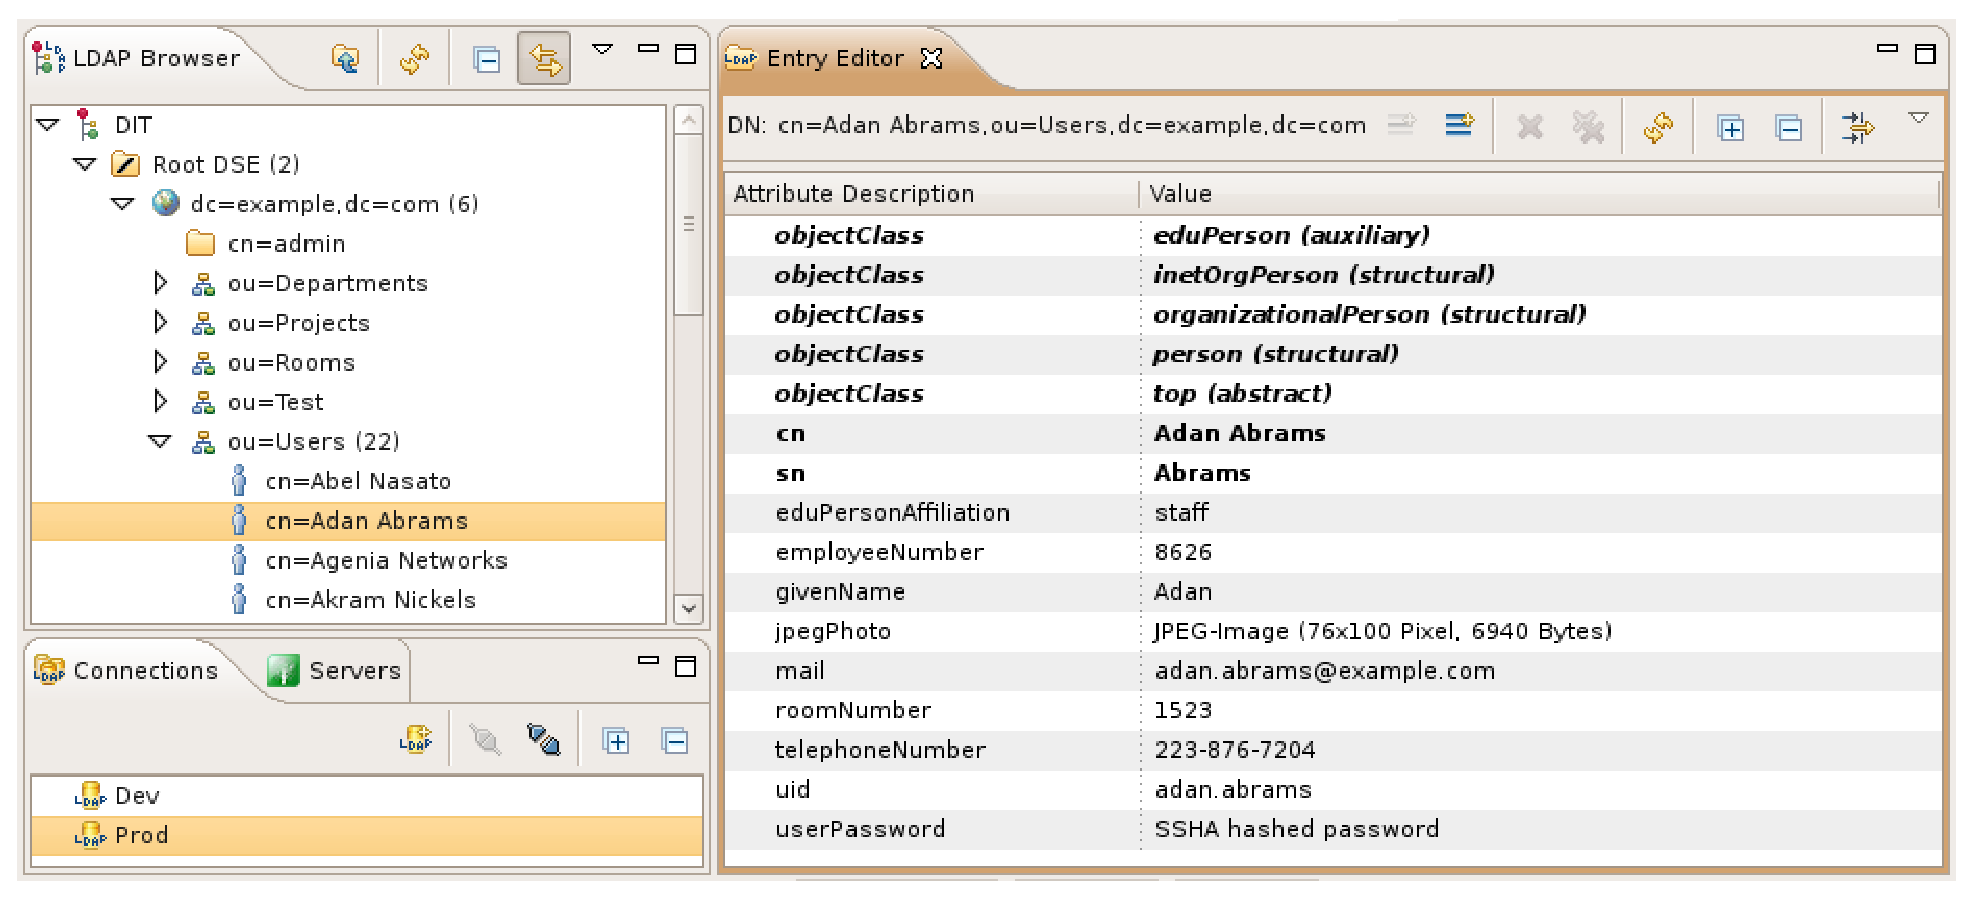
\includegraphics[width=14cm]{images/01_ldap_perspecitve.eps}
  \end{center}
  \caption{LDAP perspective}
  \label{LDAP perspective}
\end{figure}

The \textit{LDAP Browser View} shows the DIT structure of the directory server, beginning from the RootDSE. When selecting an entry, its attributes are displayed in the \textit{Entry Editor} . Different kinds of attributes (objectclass, mandatory and optional attributes) are rendered in different fonts (Figure \ref{LDAP perspective}).

A very helpful feature is the \textsc{Advanced} menu item of the context menu. It provides actions to extract particular information that is often needed in LDAP code or configuration files:
\begin{itemize}
\item DN or URL of the entry (e.g. for the search base)
\item names or values of selected attributes (e.g. all objectClass values)
\item a composed filter of selected attributes (e.g. for a search)
\end{itemize}

Querying and extracting information is a common task of LDAP applications. The powerful \textit{Search Dialog} of Apache Directory Studio helps to compose proper and efficient search queries. All search parameters can be extracted from the \textit{Search Logs View}.

A last tool to mention is the \textit{Schema Browser} which can be used to navigate through all object classes, attribute types, syntaxes and matching rules of the directory server.

\subsection{Setup LDAP Server for Development Environment}
For development and experimenting it is always useful to have a LDAP server that can be recovered from time to time. A complete LDAP server - the Apache Directory Server - is integrated and can be started, stopped and configured using a nice GUI.

\begin{figure}[htb]
  \begin{center}
  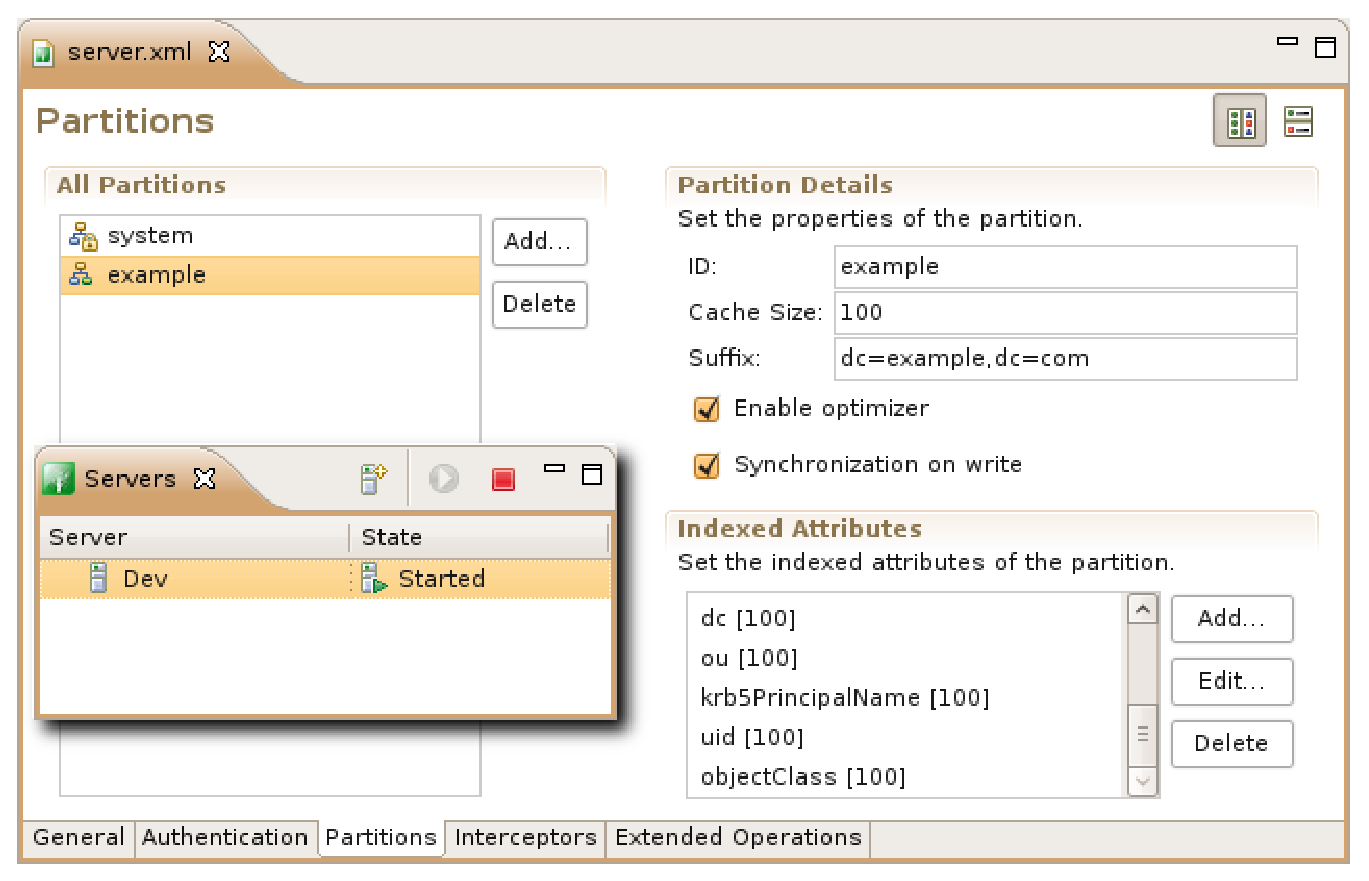
\includegraphics[width=12cm]{images/02_servers_view_and_xml.eps}
  \end{center}
  \caption{Servers view}
  \label{Servers view}
\end{figure}

Servers are managed in the \textit{Servers View} (Figure \ref{Servers view}). A new server is created by selecting \textsc{New|New Server} from the context menu and entering a name in the wizard. A double-click on the created server opens the configuration editor. The \textsc{General} tab specifies the listen ports. On the \textsc{Partitions} tab additional partitions can be added, if a new suffix is needed. After finishing the configuration the server can be started (\textsc{Run} from context menu) and a connection to this server can be created (\textsc{LDAP Browser|Create a Connection} from context menu).

\subsection{Merge Schema from Productive Server to Development Environment}
The created LDAP Server doesn't contain any data and it makes sense to copy some example data from the production server. ApacheDS is shipped with all the default schemas defined in various RFCs. However the production server contains a custom schema and it is necessary to apply this schema first.

Schemas can be managed in the \textit{Schema Editor Perspective}. The schemas of both production and the development server can be loaded by creating a new schema project of type \textit{Online Schema} and selecting the connection to the server. The \textit{Schema View} shows the available schemas and its object classes and attribute types.

To merge different schemas one must open the target schema and select \textsc{Import|Merge Schemas from other Projects} from context menu of the \textit{Schema View}. In the wizard the complete project or specific attribute types and object classes can be selected. It is recommended to only select object classes that are needed for the test data (Figure \ref{Merge schema wizard}), dependant attribute types can be merged automatically. The merged object classes and attribute types are placed in the schema named merge-of-<project name> (Figure \ref{Merged schema}). This schema can be exported to the schema format of ApacheDS (\textsc{Export|Schemas for ApacheDS} from context menu) and imported via the LDAP Browser (\textsc{Import|LDIF} from context menu). The new schema elements can be reviewed in the schema browser. Reloading the schema might be necessary using \textsc{Reload Schema} option.

\begin{figure}[htb]
 \begin{minipage}{.45\linewidth}
  \begin{center}
  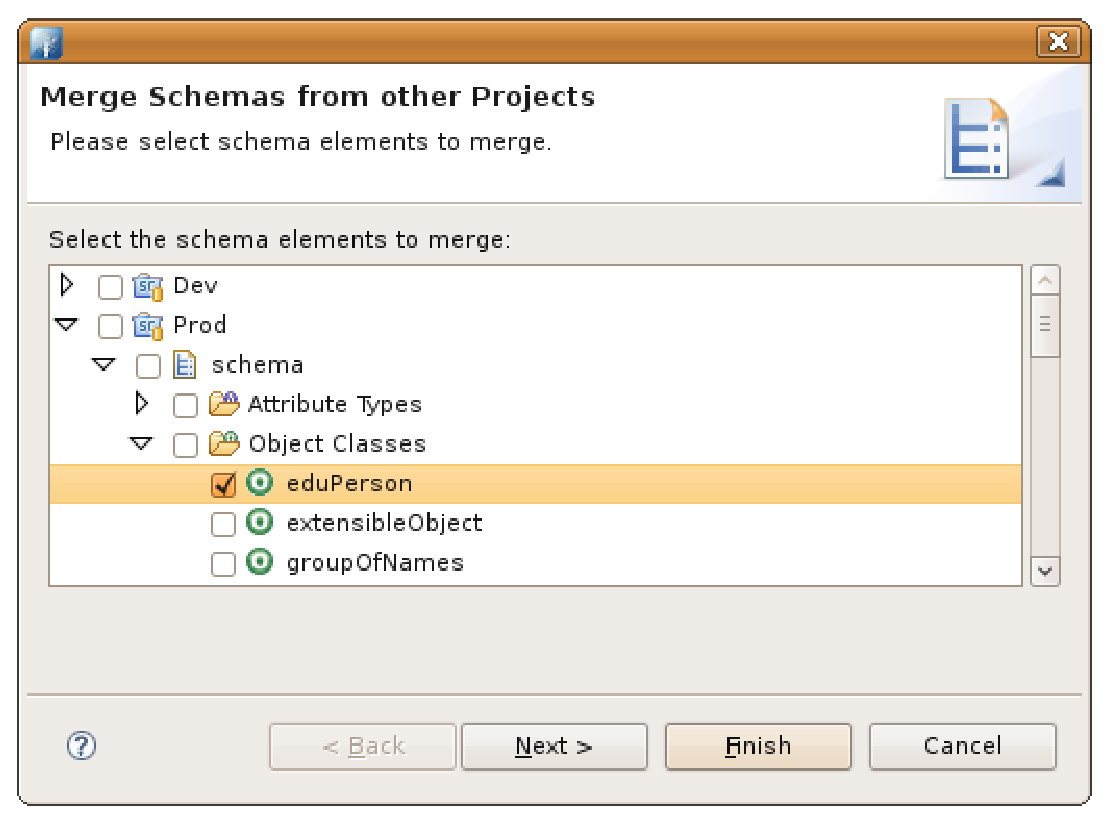
\includegraphics[width=6cm]{images/03_merge_schema_wizard.eps}
  \caption{Merge schema wizard}
  \label{Merge schema wizard}
  \end{center}
 \end{minipage}
 \hspace{.1\linewidth}% Abstand zwischen Bilder
 \begin{minipage}{.45\linewidth}
  \begin{center}
  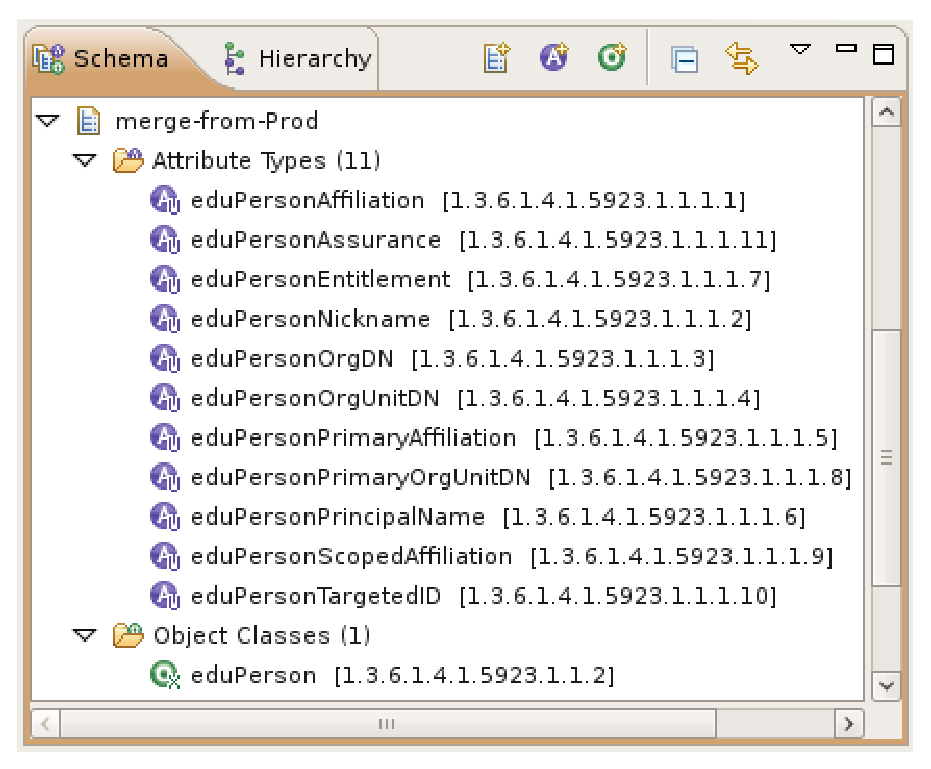
\includegraphics[width=6cm]{images/04_merge_schema_finished.eps}
  \caption{Merged schema}
  \label{Merged schema}
  \end{center}
 \end{minipage}
\end{figure}

\subsection{Copy Example Data}
The next step is to copy the DIT structure and some example data from the production server to the development server.

Select the structural entries beginning from the context entry and some data entries in the \textit{LDAP Browser View} and choose \textsc{Advanced|Copy Entry as LDIF} from context menu. Afterwards open a new LDIF editor (\textsc{File|New|LDIF File}) and paste the copied data into it (Figure \ref{Copy example data}).

If necessary the data can be modified. One feature to be mentioned here is the handling of BASE-64 encoded values. If the data contains non-ASCII characters or even binary values this data can be edited with specialized value editors. This is done by navigating the cursor to the attribute and pressing F7 or selecting \textsc{Edit Value} or \textsc{Edit Value with} from context menu.

To import the data into the development server one needs to choose a connection of the development server using the \textit{Browse...} button and hitting the \textit{Execute LDIF} button.

In the end the LDIf should be saved to disk. Later, this file can be tweaked and extended in order to create more test data. It can also be used to restore the development server to a known state.

There are two more methods worth mentioning, how to copy example data: Some single entries can just be transferd by copy/paste them. If more data is needed then it is recommended to use the powerful \textit{Export LDIF} and \textit{Import LDIF} wizards.

\begin{figure}[htb]
  \begin{center}
  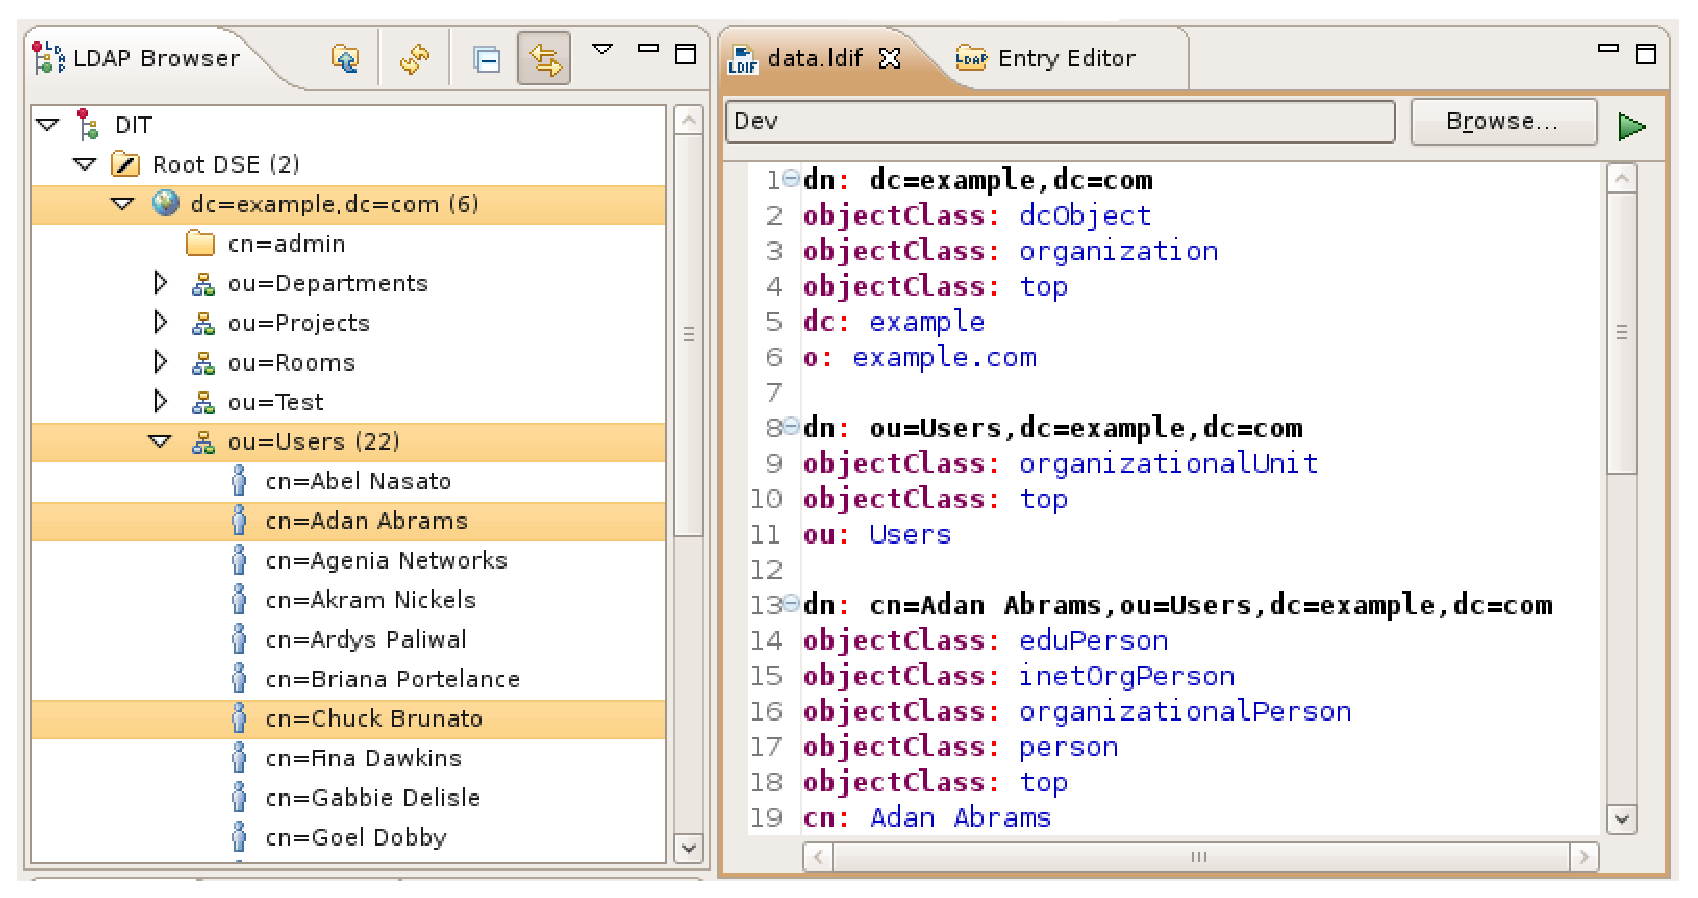
\includegraphics[width=12cm]{images/05_copy_as_ldif.eps}
  \end{center}
  \caption{Copy example data}
  \label{Copy example data}
\end{figure}

\subsection{Create a new Schema}
To be able to store objects of cars company within the directory a new schema is required. The already known \textit{Schema Editor} can be used for that. The \textit{Schema View} provides wizards for creating schema object classes and attribute types. There are editors available for editing object classes and attribute types (Figure \ref{Schema Editor perspective}). The steps to import the schema into the development server are the same as above: Export the schema in ApacheDS format and import the created LDIF. It is also possible to export the schema to other formats, like the common OpenLDAP schema file format.

\begin{figure}[htb]
  \begin{center}
  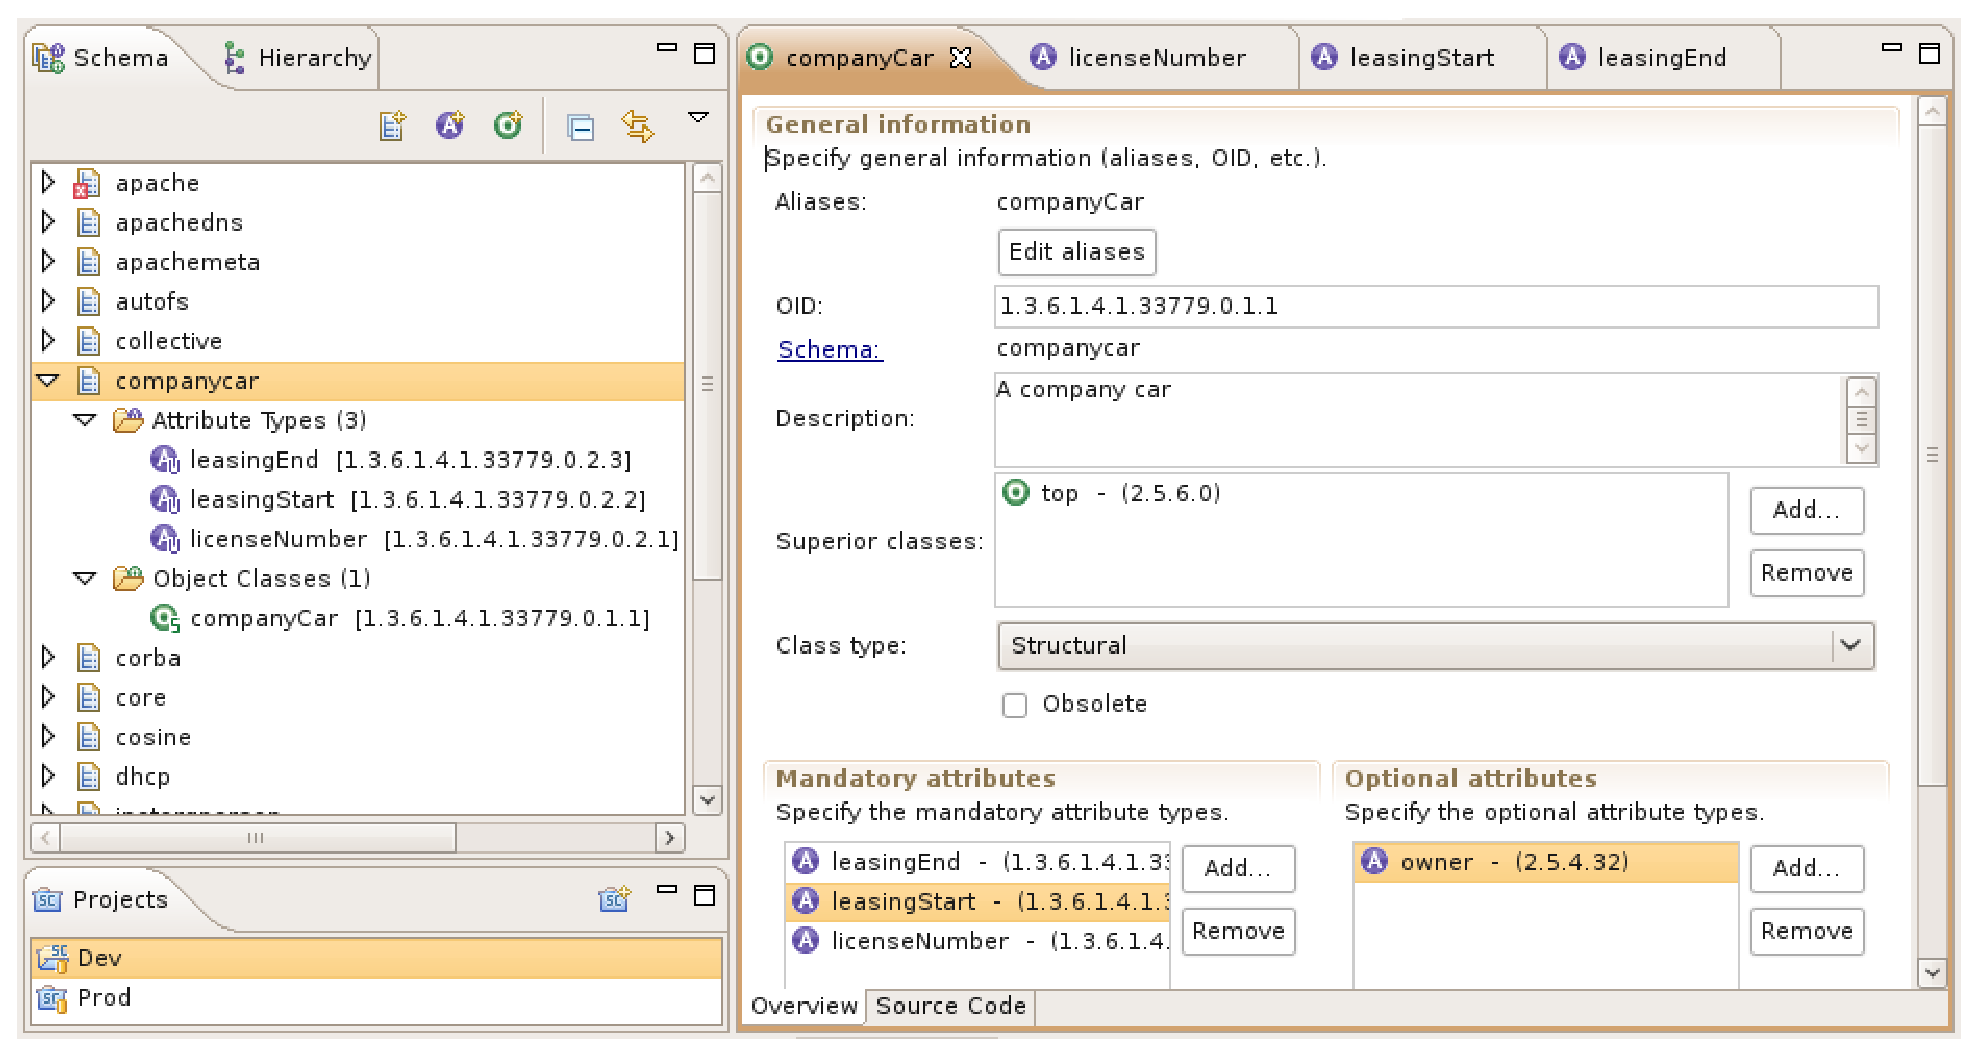
\includegraphics[width=12cm]{images/06_schema_editor.eps}
  \end{center}
  \caption{Schema Editor perspective}
  \label{Schema Editor perspective}
\end{figure}

\subsection{Unit testing}
Automated tests are essential for high-quality software development. The JUnit4 based testing framework of ApacheDS can be used to test the LDAP persistence code for Java applicaitons.

\begin{figure}[htb]
  \begin{center}
  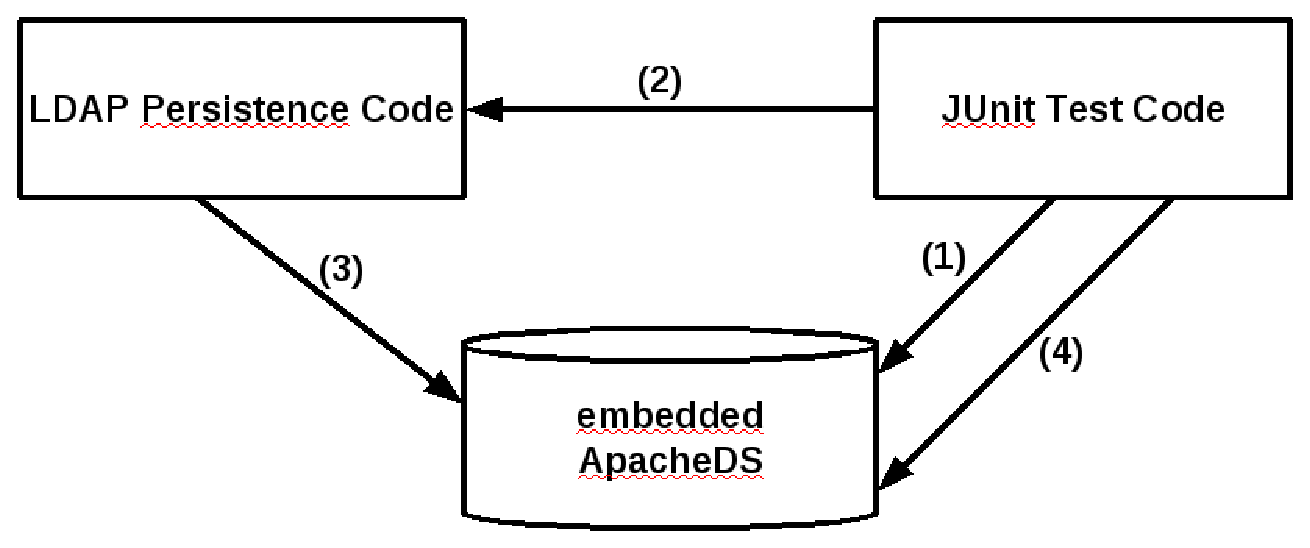
\includegraphics[width=8cm]{images/08_junit.eps}
  \end{center}
  \caption{ApacheDS testing framework}
  \label{ApacheDS testing framework}
\end{figure}

Figure \ref{ApacheDS testing framework} shows the idea behind the testing framwork. In the test code an embedded ApacheDS is started and configured (1). Then the test code invokes the persistence code (2). The persistence code either modifies data in the embedded ApacheDS or retrieves data and returns some objects to the test code. At last the test code checks that the expected modifications were done (4) or that the expected objects were returned.

\begin{SaveVerbatim}{Code1}
 1    @RunWith(SiRunner.class)
 2    @CleanupLevel(Level.METHOD)
 3    @Factory(ApacheDsFactory.class)
 4    @ApplyLdifFiles( { "/companyCar_schema.ldif", "/companyCar_data.ldif" } )
 5    public class CompanyCarDaoTest
 6    {
 7        public static LdapServer ldapServer;
 8    
 9        @Test
10        public void testPersistCompanyCar() throws Exception
11        {
12            // create the company car
13            Calendar leasingStart = Calendar.getInstance();
14            Calendar leasingEnd = Calendar.getInstance();
15            CompanyCar car = new CompanyCar( "QQ-AA-1234", leasingStart, leasingEnd );
16            CompanyCarDao dao = new CompanyCarDao();
17            dao.save( car );
18    
19            // assert the company car was created
20            Entry entry = ldapServer.getDirectoryService().getAdminSession().lookup(
21                new LdapDN( "licenseNumber=QQ-AA-1234,ou=Cars,dc=example,dc=com" ) );
22            assertNotNull( entry );
23        }
24    }
\end{SaveVerbatim}
\begin{figure}[htb]
  \fbox{
    \begin{minipage}{14.5cm}
      \scriptsize{\UseVerbatim{Code1}}
    \end{minipage}
  }
  \caption{JUnit test example}
  \label{JUnit test example}
\end{figure}

Figure \ref{JUnit test example} shows an JUnit test eample. The annotations in lines 1-4 are used to setup the embedded ApacheDS. Line 1 tells JUnit to use the custom runner which starts the embedded ApacheDS. Line 2 is used to revert modifications done by a test method to ensure the same known state for each test. Line 3 (optional) defines the factory class that starts and configures the embedded ApacheDS. Line 4 (optional) is used to inject custom schema and data into the LDAP server. The static variable \textit{ldapServer} in line 7 is injected from the framework and can be used to access the embedded LDAP server programatically. JUnit4 requires to annotate the test method (line 10-23) with \textit{@Test}. In lines 13-15 the business objects to persist are constructed. The \textit{CompanyCarDao} in line 16 contains the persistence code and in line 17 the \textit{save} method is invoked that creates an entry in the LDAP server. To check if the persistence code worked the \textit{ldapServer} object is used to lookup the created entry directly from the embedded ApacheDS (lines 20-22).

\section{Outlook}
We want to create more tools that help making LDAP more attractive for developers. New features may include code generators to create Java classes and persistence code (DAOs) from LDAP schema. The Eclipse framework also provides powerful graphical editors which can be used for schema design. 

Please join the Apache Directory community and report bugs and new ideas, participate on our mailing lists, write documentation and contribute code.

\end{document}


